\chapter{Ajuste de polinomios}

\section{El problema}
Supongamos que tenemos un conjunto de datos con solamente dos variables $x$, $y$. Buscamos ajustarlos a un polinomio de grado $k$. Es decir, buscamos ajustar los datos al modelo

\begin{equation*} 
    \begin{aligned}
    y = \sum_{j = 0}^{k} \beta_j x^j + \epsilon
    \end{aligned}
\end{equation*}

donde $j$ es el grado de la variable $x$. 

El problema consiste en encontrar los mejores coeficientes que cumplan la ecuación anterior. Una manera más compacta de ver el problema es de forma matricial 

\begin{equation}
\label{eq_matricial_pol}
    \begin{aligned}
    y = X \beta.
    \end{aligned}
\end{equation}

donde $y$ es un vector de tamaño $n$, $X$ es una matriz de tamaño $n \times (k + 1)$ y $\beta$ es un vector de tamaño $k + 1$. 

\\

\section{Los datos}
En esta sección explicare como ajustar un conjunto de datos a un polinomio de grado $k$. Los datos que usare son proporcionados por el Instituto Nacional de Standards y Tecnología (NIST por sus siglas en inglés). Para este problema, seleccioné el conjunto llamado filip que se encuentra en \url{https://www.itl.nist.gov/div898/strd/lls/data/LINKS/DATA/Filip.dat}. Estos datos contienen 82 pares ordenados $(x_i, y_i)$. La siguiente imagen muestra las primeras 10 observaciones de los datos. 

\begin{figure}[h]
\begin{center}
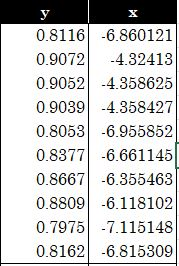
\includegraphics[scale=0.5]{Imagenes/header_filip.JPG}
  \label{header_filip}
\end{center}
\end{figure}

\valinline{no sé si agregar una gráfica rápida de los datos porque a simple vista no parecen un polinomio de grado 10}
\\
Seleccioné este conjunto de datos porque además de proporcionar la información para el ajuste, también dan la respuesta al vector $\beta$ con alta precisión en sus dígitos. 

\section{Planteamiento del problema}

De esta forma, el vector $y$ de la ecuación \ref{eq_matricial_pol} es de tamaño 82 y corresponde a la columna $y$ del conjunto de datos.
Podríamos definir la matriz $X$ de la siguiente manera

\begin{equation*}
    \begin{aligned}
    X = 
    \begin{pmatrix}
    1 & x_{1,1} & x_{1,2} & \dots & x_{1, 10}  \\
    1 & x_{2,1} & x_{2, 2} & \dots & x_{2, 10} \\
    \vdots & \vdots & \vdots & \dots & \vdots \\
    1 & x_{81,1} & x_{81, 2} & \dots & x_{81, 10} \\
    1 & x_{82,1} & x_{82, 2} & \dots & x_{82, 10}. \\
    \end{pmatrix}
    \end{aligned}
\end{equation*} 

Representar la matriz $X$ de esta forma tiene una ventaja. Cada elemento puede ser visto como $x_{i, j}$ donde el renglón $i$ representa la observación $i$ de los datos. Por otro lado, la columna $j$ representa la potencia a la que está elevada la observación $i$. Por ejemplo, el elemento $x_{34, 5}$ es la observación 34 de los datos elevado a la 5 potencia. Sin embargo, es importante reconocer que el elemento $x_{34, 5}$ realmente está en la columna 6 de la matriz. El pequeño cambio de notación es solamente para no perder de vista la potencia de las observaciones. 

\\

Por último, el vector $\beta$ de la ecuación \ref{eq_matricial_pol} es de dimensión 11 y es la incógnita del problema. 

\\

En Julia, el código para cargar los datos es el siguiente: 

\begin{minted}{julia}
    using CSV, DataFrames, Polynomials
    
    filip = CSV.read("filip_data.csv", DataFrame)

    x = filip.x
    y = filip.y
    k = 10 #grado del polinomio
    n = length(x) # número de observaciones
\end{minted}

Por otro lado, para generar la matriz X creé una función que tiene como argumento una variable $k$ que representa la potencia del polinomio que quiero ajustar. 

\begin{minted}{julia}
function generar_X(k) # k es la potencia del polinomio

    n = size(filip, 1) #numero de renglones
    
    #Defino una matriz vacía
    X = Array{Float64}(undef, n, k + 1)
    # Sabemos que la primera columna siempre es un vector de unos
    X[:, 1] = ones(n)
    
    # Para el resto de la columnas,
    # elevo cada elemento a la potencia correspondiente
    for i = 1:k
        X[:, i + 1] = x.^i
    end
    return X
end
\end{minted}


\section{Métodos}

\subsection{\textit{GLM}}

Dado que el problema es ajustar una regresión lineal, el primer paquete que se viene a la mente por utilizar es \textsf{GLM}, ya que se sus siglas se traducen a 'Modelos Lineales Generalizados'.


El manual de este paquete se puede encontrar en \url{https://juliastats.org/GLM.jl/v0.11/#Methods-applied-to-fitted-models-1}. \val{No estoy segura si dejar esto o no} 

Para ajustar un modelo lineal generalizado, hay que utilizar la función \texttt{lm(formula, data)} donde 

\begin{itemize}
    \item formula: 
    Corresponde a la fórmula del ajuste con los nombres de las columnas de los datos
    \item data:
    Debe ser un dataframe con los datos por ajustar. Los datos pueden contener valores NA. 
\end{itemize}

En nuestro caso, queremos ajustar un polinomio de grado 10 a los datos guardados con el nombre de filip. Por lo tanto, el código en Julia es

\begin{minted}{julia}
    x_fit = lm(@formula(y ~ 1 + poly(x, 10)), filip)
\end{minted}

donde \texttt{poly(x, 10)} es una función con sintaxis extendida que se utiliza específicamente para regresión polinomial. Esta función viene programada en la documentación del paquete \textsf{StatsModels} en el apartado de \textsf{Extending @formula syntax} que se encuentra en la dirección \url{https://juliastats.org/StatsModels.jl/stable/internals/}. \val{No sé si mejor poner la referencia?? creo que si}

\\

Este método no funcionó. Dado que los datos de NIST vienen con la respuesta correcta, fue claro observar que los resultados con el paquete GLM no ajustaron de manera precisa el polinomio. 

\subsection{Descomposición QR versión económica}

\begin{definition}
La factorización QR de una matriz $A$ de dimensiones $m \times n$ es el producto de una matriz $Q$ de $m \times n$ con columnas ortogonales y una matriz $R$ cuadrada y triangular superior \cite{garcia2017second}. 
\end{definition}

Una de las aplicaciones de la descomposición QR es dar solución a problemas de mínimos cuadrados. Por lo tanto, es el segundo método que utilizamos para obtener los valores $\beta$ de \ref{eq_matricial_pol}.

 \begin{definition}
 Una secuencia de vectores $u_1, u_2, \dots$ (finita o infinita) en un espacio de producto interno es ortonormal si 
 \begin{equation*}
     \begin{aligned}
     \langle u_i , uj \rangle = \delta_{ij} \text{ para toda $i, j$}
     \end{aligned}
 \end{equation*}
 Una secuencia ortonormal de vectores es un sistema ortonormal \cite{garcia2017second}.
 \end{definition}

\begin{definition}
Una base ortonormal para un espacio de producto interno finito es una base que es un sistema ortonormal \cite{garcia2017second}.
\end{definition}

En nuestro problema las dimensiones $m \times n$ de la matriz $X$ son $82 \times 11$. Además, $X$ tiene rango $r = 10 < n$ por lo que la matriz $R$ de la descomposición QR es singular. Como consecuencia, no se puede generar una base ortonormal de $R(X)$. Sin embargo, el proceso de factorización QR se puede modificar usando una matriz de permutación para generar una base ortonormal.

\\

\begin{definition}
Una matriz $A$ es una matriz de permutación si exactamente una entrada en cada renglón y en calada columna es 1 y todas las otras entradas son 0 \cite{garcia2017second}.
\end{definition}

La idea del método QR modificado es generar una matriz de permutación $P$ tal que 

\begin{equation*}
    \begin{aligned}
    AP = QR
    \end{aligned}
\end{equation*}

donde 

\begin{equation*}
    \begin{aligned}
    R = 
    \begin{pmatrix}
    R_{11} & R_{12} \\
    0      & 0
    \end{pmatrix}
    \end{aligned}
\end{equation*}

En este caso, si tomamos $r$ como el rango de $X$ entonces $R_{11}$ es de dimensión $r \times r$ triangular superior y $Q$ es ortogonal. Las primeras $r$ columnas de $Q$ forman una base ortonormal de $R(X)$ \cite{numerical_linear_algebra}. La factorización QR con columnas pivoteadas \val{si se dice asi? le dicen version economica en el articulo pero no encuentro la traduccion} siempre existe debido al siguiente teorema.

\begin{theorem} \label{exitencia_QR_dec}
Sea $A$ una matriz de $m \times n$ con rango($A$) = $r \leq min (m, n)$. Entonces, existe una matriz de permutación $P$ de $n \times n$ y una matriz ortogonal $Q$ de dimensiones $m \times m$ tal que 
\begin{equation*}
\begin{aligned}
Q^{T}AP = 
\begin{pmatrix}
R_{11} & R_{12} \\
   0      & 0
\end{pmatrix}
\end{aligned}
\end{equation*}
donde $R_{11}$ es una matriz triangular superior de tamaño $r \times r$ con entradas en la diagonal diferentes de cero. 
\end{theorem}

\cite{numerical_linear_algebra}

\val{literal el teorema viene de Datta 2010}

Para aplicar este método en Julia, hay que usar el siguiente código

\begin{minted}{julia}
    ### Con QR Pivoted
    F = qr(X, Val(true))
    Q = F.Q
    P = F.P
    R = F.R
\end{minted}

\\

Ya tenemos el código que calcula las matrices $P, Q, R$ de la descomposición QR con columnas pivoteadas. Para resolver nuestro problema original \ref{eq_matricial_pol} y obtener los valores de los elementos de $\beta$ hay que hacer un poco de álgebra. 

\\

Recordemos que el problema es obtener $\beta$ de la ecuación $y = X \beta$. También, por el teorema \ref{exitencia_QR_dec}, sabemos que $X$ siempre tiene descomposición QR con columnas pivoteadas. Es decir, $XP = QR$. Por otro lado, como $P$ es matriz de permutación por lo que

\begin{equation*}
    \begin{aligned}
    \exists z \text{ tal que } Pz = \beta .
    \end{aligned}
\end{equation*}

Por lo tanto, ya tenemos una expresión para $\beta$ que podemos sustituir en la ecuación \ref{eq_matricial_pol} para obtener 
\begin{equation*}
    \begin{aligned}
    y = X (Pz) . 
    \end{aligned}
\end{equation*}

A la vez, sustituyendo en la fórmula de la descomposición QR

\begin{equation*}
    \begin{aligned}
    (XP) z = (QR) z . 
    \end{aligned}
\end{equation*}

Uniendo las dos ecuaciones anteriores, obtenemos 

\begin{equation*}
    \begin{aligned}
    y = XP z = QR z 
    \longrightarrow y = QRz
    \end{aligned}
\end{equation*}

Por lo tanto, el primer paso es resolver la ecuación 

\begin{equation*}
    \begin{aligned}
    y = QRz
    \end{aligned}
\end{equation*}

Para finalmente obtener $\beta$ calculando 
\begin{equation*}
    \begin{aligned}
    \beta = Pz
    \end{aligned}
\end{equation*}

En Julia, esto se programa de la siguiente manera
\begin{minted}{julia}
    # 1. Resolver QRz = y
    z = Q*R \ y
    # 2. Resuelvo beta = Pz
    x_QR = P*z
\end{minted}
\\

Este método tampoco funcionó. Podemos empezar a consider que los datos son tan sensibles que la propagación del error es tal que no permite un buen ajuste del polinomio. Intentaremos con otros dos métodos.

\subsection{Descomposición de valores singulares}

La tercer manera en la que intenté resolver este problema fue usando la descomposición de valores singulares para obtener la matriz pseudoinversa de Moore-Penrose. 

\begin{definition}
Sea $A$ una matriz de $m \times n$ y sea $q = min \{m, n \}$. Si el rango de $A = r \geq 1$, sean $\sigma_1 \geq \sigma_2 \geq \dots \geq \sigma_r > 0$ los eigenvalores positivos en orden decreciente de $(A^{*}A)^{1/2}$. Los valores singulares de $A$ son
\begin{equation*}
    \begin{aligned}
    \sigma_1, \sigma_2, \dots, \sigma_r \text{ y } \sigma_{r+1} = \sigma_{r+2} = \dots = \sigma_q = 0.
    \end{aligned}
\end{equation*}
Si A = 0, entonces los valores singulares de A son $\sigma_1 = \sigma_2 = \dots = \sigma_q = 0$. 
Los valores singulares de $A \in M_{n}$ son los eigenvalores de $(A^{*}A)^{1/2}$ que son los mismos eignevalores de $(AA^{*})^{1/2}$
\cite{garcia2017second}
\end{definition}

Los valores singulares tienen muchas apliciones. Sin embargo, para resolver ecuaciones lineales son usados para obtener la descomposición de valores singulares (DVS). 


\begin{theorem}
Sea $A \in M_{m \times n} (F)$ diferente de cero y sea $r =   rango(A)$. Sean $\sigma_1 \geq \sigma_2 \geq \dots \geq \sigma_r > 0$ los valores singulares positivos de A y definamos

\begin{equation*}
    \begin{aligned}
    \Sigma_r = 
    \begin{pmatrix}
    \sigma_1 & & 0 \\
     & \ddots & & \\
     0 & & \sigma_r
    \end{pmatrix}
    \in M_{r}(R).
    \end{aligned}
\end{equation*}
Entonces, existen matrices unitarias $U \in M_{m}(F)$ y $V \in M_{n}(F)$ tales que 
\begin{equation} \label{decomposicion}
    \begin{aligned}
    A = U \Sigma V^{*}
    \end{aligned}
\end{equation}
donde
\begin{equation*}
    \begin{aligned}
    \Sigma = 
    \begin{pmatrix}
    \Sigma_r & 0_{r \times (n-r)} \\
    0_{(m-r) \times r} & 0_{(m-r) \times (n-r)}
    \end{pmatrix}
    \in M_{m \times n}(R)
    \end{aligned}
\end{equation*}
 tiene las mismas dimensiones que A. Si m = n, entonces $U, V \in M_{n}(F)$ y $\Sigma = \Sigma_r \oplus 0_{n-r}$.
 \cite{garcia2017second}
\end{theorem}

La ecuación \ref{decomposicion} con las características del teorema anterior lleva por nombre descomposición en valores singulares (DVS). 

\\

Es importante observar que las matrices $U$ y $V$ son matrices unitarias. Es decir, 

\begin{equation*}
    \begin{aligned}
    U U^{*} u = u, \text{ } \forall u \in Col (U)
    \end{aligned}
\end{equation*}

\begin{equation*}
    \begin{aligned}
    V V^{*} v = v, \text{ } \forall v \in Col (V)
    \end{aligned}
\end{equation*}

\subsubsection{Pseudoinversa de Moore-Penrose}

Ya que conocemos la descomposición de valores singulares, podemos avanzar y definir la descomposición de valores singulares para la pseudoinversa de Moore Penrose. 

\begin{theorem}
Sea $A$ una matriz de $m \times n$ de rango $r$ con una descomposición en valores singulares de $A = U \Sigma V^{*}$ y valores singulares diferentes de cero $\sigma_1 \geq \sigma_2 \geq \dots \geq \sigma_r$. Sea $\Sigma^{\dagger}$ una matriz de $n \times m$ definida como
\begin{equation*}
    \begin{aligned}
   \Sigma^{\dagger}_{ij} =
   \begin{cases}
   \dfrac{1}{\sigma_i} \text{ si } i = j \leq r\\
   0 \text{ en otro caso.}
   \end{cases}
    \end{aligned}
\end{equation*}
Entonces $A^{\dagger} = V \Sigma^{\dagger} U ^{*}$ y esta es la descomposición de valores singulares de $A^{\dagger}$. 
\cite{friedberglinearalgebra}
\end{theorem}

Podemos ver que en realidad lo único que cambia al calcular la pseudoinversa es la matriz $\Sigma$. Sin embargo, esta nueva matriz $A^{\dagger}$ tiene propiedades interesantes. 

\begin{itemize}
    \item $(A^{T}A)^{\dagger} A^{T} = A^{\dagger}$
    \item $(AA^{T})^{\dagger} A = (A^{\dagger})^{T}$
    \item $(A^{T}A)^{\dagger}(A^{T}A) = A^{\dagger}A = VV^{T}$
\end{itemize}


Recordando que buscamos obtener $\beta$ que satisfaga la ecuación \ref{eq_matricial_pol} podemos ver que el sistema lineal está sobredeterminado. Esto se puede verificar por las dimensiones de la matriz $X_{n \times m} = X_{82 \times 11}$. Como $m < n$, sabemos que hay más ecuaciones que variables desconocidas. 

\\

\valinline{Como sabemos que y esta en el espacio de columnas de V?}
De la ecuación \ref{eq_matricial_pol} podemos multiplicar por $X^{T}$ para obtener

\begin{equation}
\label{transformacion_eq_base}
    \begin{aligned}
    X^{T}X \beta = X^{T} y, \text{ } y \in Col(V).
    \end{aligned}
\end{equation}

La ecuación \ref{transformacion_eq_base} siempre da un sistema determinado (balanceado) \cite{worldScientificNews}. Ahora bien, multiplicando \ref{transformacion_eq_base} por $(X^{T}X)^{\dagger}$ y usando las propiedades de la matriz pseudo inversa podemos obtener 


\begin{equation*}
    \begin{aligned}
    (X^{T}X)^{\dagger} X^{T}X \beta = (X^{T}X)^{\dagger} X^{T} y \\
    \iff X^{\dagger} X \beta = X^{\dagger} y \\
    \iff V V^{T} \beta = X^{\dagger} y \\
    \beta = X^{\dagger} y 
    \end{aligned}
\end{equation*}. 

Por lo tanto, la pseudo inversa de Moore Penrose da la solución de mínimos cuadrados de \ref{eq_matricial_pol} \cite{worldScientificNews}

\\

En Julia, este método se puede programar de la siguiente manera:

\begin{minted}{julia}
    ### Inversa de Moore Penrose
    N = pinv(X)
    aux = ones(k + 1)
    x_MP = N*y 
\end{minted}

Este método tampoco funcionó. Por lo tanto, investigue más a fondo los paquetes de Julia hasta encontrar el paquete \textit{Polynomials}. 

\subsection{\textit{Polynomials}}
\textit{Polynomials} es un paquete que proporciona aritmética básica, integración, diferenciación, evaluación y hallar raíces para polinomios univariados \cite{poly_manual}. Para poder usar el paquete primero hay que descargarlo usando el código \ref{instalacion_paquete}. 

\\

El paquete \textit{Polynomials} tiene su propia función \texttt{fit} que toma tres variables como entrada. Las primeras dos entradas son las correspondientes a $x$ y $y$ de los datos a utilizar (en este caso, los datos filip). La tercera entrada corresponde al grado que buscamos que sea el polinomio (en este caso, grado 10). 

\\

A diferencia de los otros método utilizados para este problema, la función \texttt{fit} usa el metódo Gauss-Newton para resolver sistemas de ecuaciones no lineales. Sin embargo, en este caso tenemos un problema lineal. Esta fue la primera razón por la que este paquete no fue mi primera opción para resolver el problema. 
\valinline{No sé si tengo que explicar este método}

\\

La segunda razón es que a diferencia de la función \texttt{lm} del paquete \textit{GLM}, la función \texttt{fit} solamente aporta los coeficientes del ajuste del polinomio. Es decir, no da como resultado el error estandar, ni el valor p de la estimación. Sin embargo, tengo que agregarlo a esta sección de la tesis, ya que es el único método que funcionó. 

\\

El código en Julia se ve de la siguiente manera:

\begin{minted}{julia}
using Polynomials 
x_pol = Polynomials.fit(x, y, 10)
\end{minted}

\\

Este método fue el único de los cuatro que funcionó para el polinomio de grado 10. La desventaja de este método es que la función solamente arroja los coeficientes $\beta$. Si quisieramos ampliar el análisis y observar, por ejemplo, el valor p de algún regresor tendríamos que buscar otra manera de obtenerlo. 


\section{Evaluación de los métodos}
Una cuestión válida es preguntarse si tal vez lo que está mal es la implementación de los algoritmos y, debido a esto, no dan la respuesta correcta. Por tanto, para probar que los métodos estén programados de la manera correcta los somentí a una serie de pruebas.

\\

La primera prueba consiste en que, usando los datos filip, cada método ajustaba un polinomio de grado $k$ de $k = 1, 2, \dots, 10$. Al final, para cada polinomio de grado $k$ tenía cuatro resultados de ajuste (uno por cada método). 

\\

La segunda prueba consiste en comparar los resultados con R. De manera análoga a Julia, en R también use los datos filip para ajustar un polinomio de grado $k$ de $k = 1, 2, \dots, 10$. Para esto, use la función \texttt{lm(formula, data)} donde los datos siempre son los mismos y la fórmula depende del grado del polinomio. La tercera prueba fue medir el tiempo que tomaba a R ejecutar la función \texttt{lm} con los parametros especificados. El código es el siguiente: 

\begin{minted} {R}
# Para polinomio de grado = 1
start <- Sys.time()
lm_1 <- lm(y ~ x, data = data, x = TRUE)
end <- Sys.time()

`resultados_grado_ 1`$R <- lm_1$coefficients
row.names(`resultados_grado_ 1`) <- c("b0", "b1")
X_1 <- lm_1$x

time_vec <- c(end - start)

# Para polinomios de grado > 1

for (i in 2:10){
  #Hacemos el modelo
  model <- paste("y ~ x", paste("+ I(x^", 2:i, ")", sep='', collapse=''))
  
  # Lo convertimos en formula
  form <- formula(model)
  
  #Ejecutamos el modelo
  start <- Sys.time()
  lm.plus <- lm(form, data = data, x = TRUE)
  end <- Sys.time()
  time <- end - start
  time_vec <- c(time_vec, time)
  
  # Guardo el df correspondiente a un auxiliar
  resultados_aux <- get(paste("resultados_grado_", i))
  # para unirle los coeficientes
  resultados_aux$R <- lm.plus$coefficients
  
  nombres <- c("b0")
  # Para el nombre de los renglones
  for (k in 1:i){
    nombres <- c(nombres, paste0("b", k))
  }
  row.names(resultados_aux) <- nombres
  
  #Finalmente, hago el df final
  assign(paste("resultados_grado_", i), resultados_aux)
  
  assign(paste("X_", i), lm.plus$x)
 
\end{minted}

No voy a mostrar todas las tablas con los resultados ya que son muchas. Me voy a limitar a las tablas que considero tienen los resultados más relevantes. Para el polinomio de grado 1, todos los métodos obtienen los mismos resultados. 

\begin{figure}[h]
\begin{center}
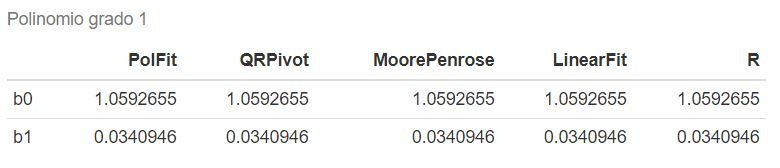
\includegraphics[scale=0.5]{Imagenes/tabla_pol_1.JPG}
\end{center}
\end{figure}

Todos los métodos funcionan bien calculando el ajuste hasta llegar al polinomio de grado 5. Cuando calculamos el polinomio de grado 6, el método \texttt{fit} del paquete \texttt{GLM} llamado \texttt{LinearFit} comienza a fallar. 

\begin{figure}[h]
\begin{center}
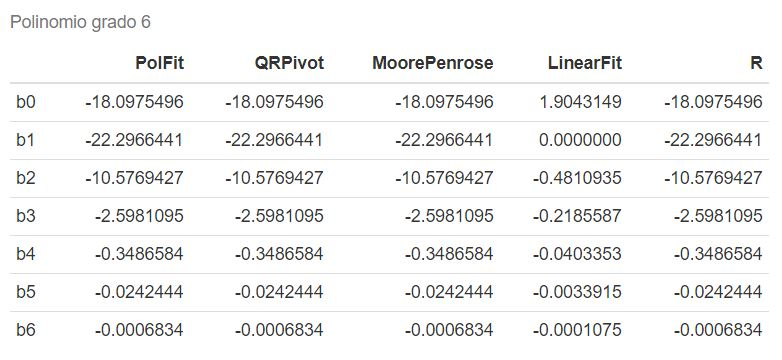
\includegraphics[scale=0.5]{Imagenes/tabla_pol_6.JPG}
\end{center}
\end{figure}

A partir del polinomio de grado 6, \texttt{LinearFit} comienza a fallar y comienza a dar resultados muy érroneos. Todos los métodos arrojan resultados correctos hasta que llegamos al polinomio de grado 10. 

\begin{figure}[h]
\begin{center}
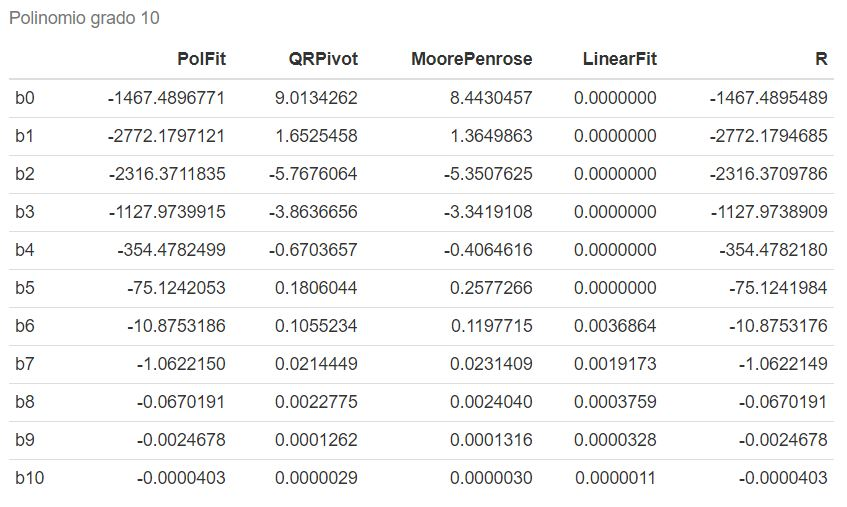
\includegraphics[scale=0.5]{Imagenes/tabla_pol_10.JPG}
\end{center}
\end{figure}

Finalmente, podemos ver la tabla de tiempos que le tomo a cada método. Las columnas representan los métodos usados mientras que los renglones el grado de polinomio que se ajustó. 

\begin{figure}[h]
\begin{center}
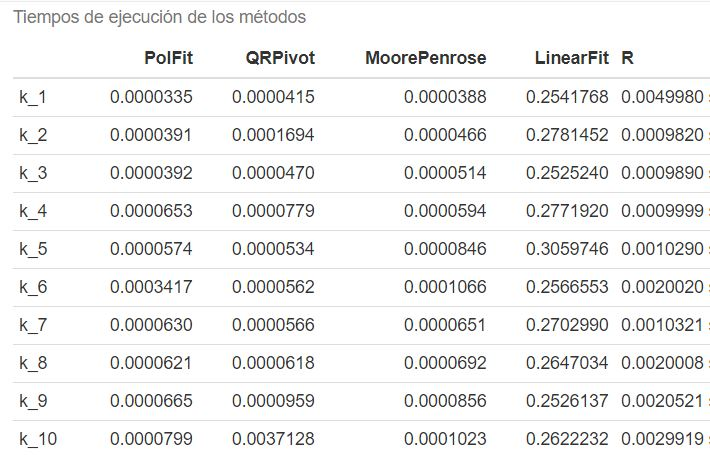
\includegraphics[scale=0.5]{Imagenes/table_tiempos.JPG}
\end{center}
\end{figure}

\valinline{Las tablas están por donde quieren, mejor copio los resultados?}



\section{Eigenvalores y valores singulares}
\valinline{No estoy segura de que poner dado que no sale la igualdad basica entre eigenvalores y valores singulares}

\section{Número de condición y precisión de la solución}

\begin{definition}
El número $\parallel A \parallel  \parallel A^{-1} \parallel$ se llama el número de condición de $A$ y se denota $Cond(A)$ \cite{numerical_linear_algebra}. 
\end{definition}

Como vimos en la sección de Evaluación de los métodos, los métodos sí están bien programados. Dejando de lado las funciones programadas por default en Julia, el método de factorización QR y descomposición de valores singulares arrojaron buenos resultados hasta los polinomios de grado 9. Esto nos puede llevar a pensar que en realidad, los datos en sí son muy susceptibles a cambios. Es decir, cualquier cambio en la matriz $X$ o en el vector $y$ resultara en un ajuste de los coeficientes $\beta$ poco preciso. Esta cualidad también se conoce como que los datos tienen impurezas. El caso contrario, donde los métodos dan resultados precisos se conoce a los datos como exactos \cite{numerical_linear_algebra}.

\\

En general, para nuestro problema \ref{eq_matricial_pol} tenemos tres casos: 
\begin{itemize}
    \item El vector $y$ tiene impurezas mientras que la matriz $X$ es exacta.
    
    \item La matriz $X$ tiene impurezas mientras que el vector $y$ es exacto
    
    \item Ambos, el vector $y$ y la matriz $X$ tiene impurezas. 
\end{itemize}

En nuestro caso, nos vamos a enfocar en el tercer caso ya que no tenemos razón para pensar que solamente una columna de los datos originales tiene impurezas mientras que la otra no. 


\begin{theorem} \label{teo:perturbaciones}
Supongamos que queremos resolver el sistema $Ax = b$. Supongamos que $A$ es no singular, $b \neq 0$, y $\parallel \Delta A \parallel < \dfrac{1}{\parallel A^{-1} \parallel}$. Entonces
\begin{equation*}
    \begin{aligned}
    \dfrac{\parallel \delta x \parallel}{\parallel x \parallel} \leq (\dfrac{Cond(A)}{1 - Cond(A) \dfrac{\parallel \Delta A \parallel}{\parallel A \parallel}}) (\dfrac{\parallel \Delta A \parallel}{\parallel A \parallel} + \dfrac{\parallel \delta b \parallel}{\parallel b \parallel})
    \end{aligned}
\end{equation*} \cite{numerical_linear_algebra}
\end{theorem}

El teorema anterior nos está diciendo que los cambios en la solución $x$ son menor o iguales a una constante determinada por el número de condición multiplicada por la suma de las pertubaciones de $A$ y las pertubaciones de $b$. Además, el teorema nos dice que aunque las perturbaciones de $A$ y $b$ son pequeñas, puede haber un cambio grande en la solución si el número de condición es grande. Por lo tanto, $Cond(A)$ juega un papel crucial en la sensibilidad de la solución \cite{numerical_linear_algebra}. 

\\

El número de condición tiene varias propiedades pero en la que nos queremos centrar es en la siguiente: 

\begin{equation} \label{formula:num_cond}
    \begin{aligned}
    Cond(A) = \dfrac{\sigma_{máx}}{\sigma_{mín}}
    \end{aligned}
\end{equation}

donde $\sigma_{max}$ y $\sigma_{mín}$ son, respectivamente, el valor singular más grande y más pequeño de $A$. 

\\

Antes de calcular el número de condición de nuestra matriz $X$ de \ref{eq_matricial_pol}, vamos a ver una última definición. 

\begin{definition} \label{def:condicionamiento}
El sistema $Ax = b$ está mal condicionado si el $Cond(A)$ es grande (por ejemplo, $10^{5}, 10^{8}, 10^{10}, etc)$. En otro caso, está bien condicionado \cite{numerical_linear_algebra}.
\end{definition}

Ahora vamos a calcular el número de condición. Este calculo lo hice en Julia y en R usando ambos, la función que ya viene programada en cada lenguaje y usando la fórmula \ref{formula:num_cond}. En Julia, el código es 

\begin{minted}{julia}
# Con función de Julia
numcond_1 = cond(X_10)

# Usando propiedad de valores singulares
sing_values = svd(X_10).S
sing_values = sort(sing_values)
numcond_2 = sing_values[length(sing_values)] / sing_values[1]
\end{minted}

Los resultados son $numcond_1 = 1.7679692504686805e15$ y $numcond_2 = 1.7679692504686795e15$. Por otro lado, en R el código es 

\begin{minted}{R}
# con función de R
numcond_R1 <- cond(X)

# Usando propiedad de valores singulares
S.svd <- svd(X)
S.d <- S.svd$d
S.d <- sort(S.d, decreasing = TRUE)
numcond_R2 <- S.d[1] / S.d[length(S.d)]
\end{minted}

Los resultados son $numcond_{R1} = numcond_{R2} = 1.767962e{15}$. En conclusión, en ambos lenguajes cualquier método confirma que el número de condición de la matriz $X$ de \ref{eq_matricial_pol} es bastante grande por lo que por \ref{def:condicionamiento} sabemos que nuestro problema está mal condicionado. \valinline{Tengo duda, entonces alguien me podría decir que para que los uso}







